\newcommand\bildzrange{%
\begin{tikzpicture}[overlay, remember picture]
   \node[inner sep=0pt,below right] (image) at ([xshift=-10cm,yshift=-3.1cm]current page.north east)
  {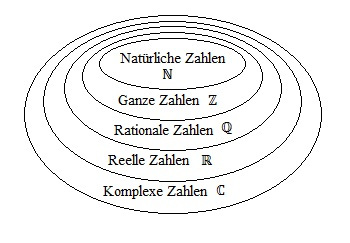
\includegraphics[width=7.5cm,height=4.1cm]{pics/zbereiche.jpg}};
\end{tikzpicture}}

\newcommand\legendezbereiche{%
\begin{tabular}{ll}
 $\mathbb{C}$  & = komplexe Zahl    \\
 $\mathbb{I}$  & = irrationale Zahl \\
 $\mathbb{N}$  & = natürliche Zahl  \\
 $\mathbb{Q}$  & = rationale Zahl   \\
 $\mathbb{R}$  & = reelle Zahl      \\
 $\mathbb{Z}$  & = ganze Zahl       \\
\end{tabular}
\\
\begin{tabular}{ll}
 $ f $         & = Funktion \\
 $ x $         & = Argument, x-Wert, unabhängige Variable  \\
 $ y $         & = Funktionswert, y-Wert, abhängige Variable  \\
 $ y = f(x) $  & = Funktionsgleichung, Zuordnungsvorschrift  \\
 $ f(x) $      & = spricht man ''f von x'' \\
 $ D \: (oder \: \mathbb{D} ) $ & = Definitionsmenge, Definitionsbereich  \\
 $ W $         & = Wertemenge, Wertebereich \\
 & \\
 $ f(x) = c $  & = konstante Funktion \\
 $ f(x) = mx + n $ & = lineare Funktion \\
 $ f(x) = ax^2 + bx + c $ & = quadratische Funktion \\
 $ f(x) = \frac{a_n x^a_n + a_n -1^{x^{n-1}} + \ldots + a_1 x + a_0}{a_m x^m + b_m -1^{x^{m-1}} + \ldots + b_1 x + b_0} $ &
 = rationale gebrochene Funktion
\end{tabular}}

